\newif\ifglobal

%%%%%%%%%%%%%%%%%%%%%%%
%%% Compile to view %%%
%%%%%%%%%%%%%%%%%%%%%%%

%%%%%%%%%%%%%%%%%%%%%%%%%%%%%%%%%%%%%%%%%%%%%%%%%%%
%%% Readme:                                     %%%
%%% https://www.overleaf.com/read/bwdjvfjksvjy/ %%%
%%%%%%%%%%%%%%%%%%%%%%%%%%%%%%%%%%%%%%%%%%%%%%%%%%%

% >>> M?: marks a module setting number or important notice

% >>> M4: Set {./relative-path} to external files for this module <<<
\def \modulefiles {./16-IOMUXGPIO}
% To add an external file, use:
% (Replace '---' with actual filename)
% '\input{\modulefiles/tables/---.tex}' for tables
% '\includegraphics{\modulefiles/figures/---}' for figures
% '\subfile{\modulefiles/---}' for register files


% >>> M1: This module is in global project? <<<
% 'YES' - uncomment; 'NO' - comment out
\globaltrue

\ifglobal
    \documentclass[main\_\_CN.tex]{subfiles}
   
\else
    % Font "FandolSong-Regular" used by ctex does not have GSUB table.
    % It causes warnings that do not affect compilation and can be ignored.
    \PassOptionsToPackage{quiet}{fontspec}

    \documentclass[openany, 10pt]{book}
   
    % >>> M2: In ./00-shared/preamble-trm-module, also find
    %         settings for visibility of todo notes, watermark <<< 
    \usepackage{preamble-trm-module}


    % Enable Chinese typesetting
    \usepackage{ctex}

    % >>> M3: Temporary labels in Chinese
    %         you can add your own labels there <<<
    \myexternaldocument{./00-shared/temp-labels-cn}

\fi %\ifglobal


\setcounter{secnumdepth}{4}


% >>> M5: If this module needs any updates in
% './00-shared/preamble-trm-module.sty'
% (include additional package, etc.), contact your module PM
% or create the file './00-shared/changelog.tex' make the
% necessary updates yourself and document them in this file <<<


\begin{document}


% Sets language into which pre-defined bits of text are translated
\selectlanguage{chinese}

% Do not delete this block
\ifglobal
% Add the following front matter if
% this module is outside of global project
\else
    \InputIfFileExists{readme}{}{}
    {\let\clearpage\relax \listoftodos}
    \tableofcontents
    %\listoftables
    %\listoffigures
\fi
%%%%%%%%%%%%%%%%%%%%%%%%%
%%% TRM Module Begins %%%
%%%%%%%%%%%%%%%%%%%%%%%%%

\hypertarget{iomuxgpio}{}
\chapter{IO MUX 和 GPIO 交换矩阵 (GPIO, IO MUX)}
\label{mod:iomuxgpio}

\section{概述}

\chipname{} 芯片有 22 个物理通用输入输出管脚 (GPIO Pin)。每个管脚都可用作一个通用 IO，或连接一个内部的外设信号。利用 GPIO 交换矩阵和 IO MUX，可配置外设模块的输入信号来源于任何的 IO 管脚，并且外设模块的输出信号也可连接到任意 IO 管脚。这些模块共同组成了芯片的 IO 控制。

{\bfseries 注意：这 22 个物理 GPIO 管脚的编号为：0 \verb+~+ 21。}

\section{主要特性}

\textbf{GPIO 交换矩阵主要特性}

\begin{itemize}
\item GPIO 交换矩阵是外设输入输出信号和 GPIO 管脚之间的全交换矩阵；
\item 42 个外设输入信号可以选择任意一个 GPIO 管脚的输入信号；
\item 每个 GPIO 管脚的输出信号可以来自 78 个外设输出信号的任意一个；
\item 支持输入信号经 GPIO SYNC 模块同步至 APB 时钟总线；
\item 支持输入信号滤波；
\item 支持 Sigma Delta 调制输出 (SDM)；
\item 支持 GPIO 简单输入输出。
\end{itemize}

\textbf{IO MUX 主要特性}

\begin{itemize}
\item 为每个 GPIO 管脚提供一个寄存器 \hyperref[regdesc:IOMUXGPIONREG]{IO\_MUX\_GPIO\regindex{n}\_REG}，每个管脚可配置成：
    \begin{itemize}
        \item GPIO 功能，连接 GPIO 交换矩阵；
        \item 直连功能，旁路 GPIO 交换矩阵。
    \end{itemize}
\item 支持快速信号如 SPI、JTAG、UART 等可以旁路 GPIO 交换矩阵以实现更好的高频数字特性。所以高速信号会直接通过 IO MUX 输入和输出。 
\end{itemize}

\section{结构概览}
本小节主要介绍 IO MUX 以及 GPIO 交换矩阵的架构，其中：
\begin{itemize}
    \item 图 \ref{fig:iomux-gpio-matrix-overview} 简要展示了 IO MUX 和 GPIO 交换矩阵的工作流程；
    
    \item 图 \ref{fig:iomux-gpio-matrix-overview-detail} 详细展示了 IO MUX 和 GPIO 交换矩阵将信号引入外设和引出至管脚的具体过程；
    
    \item 图 \ref{fig:pad-overview} 展示了 GPIO 管脚的接口逻辑。
\end{itemize}

\begin{figure}[H]
    \centering
    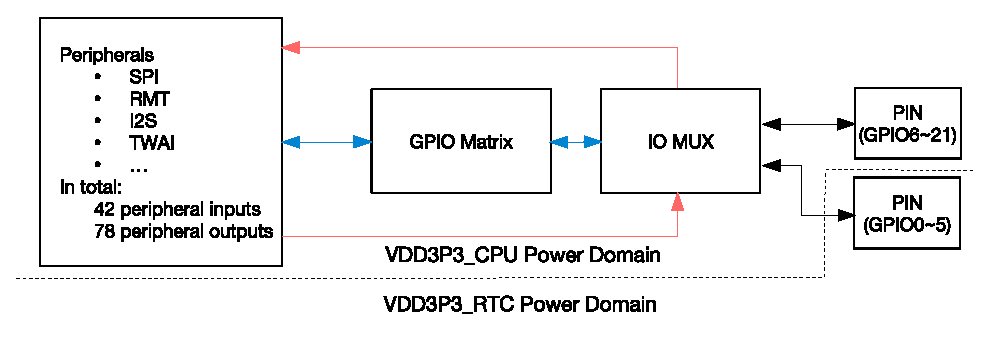
\includegraphics[width=1.0\textwidth]{16-IOMUXGPIO/figures/figure1-overview-simple-20210803}
    \caption{IO MUX 和 GPIO 交换矩阵框图（简图）}
    \label{fig:iomux-gpio-matrix-overview}
\end{figure}

\begin{figure}[H]
    \centering
    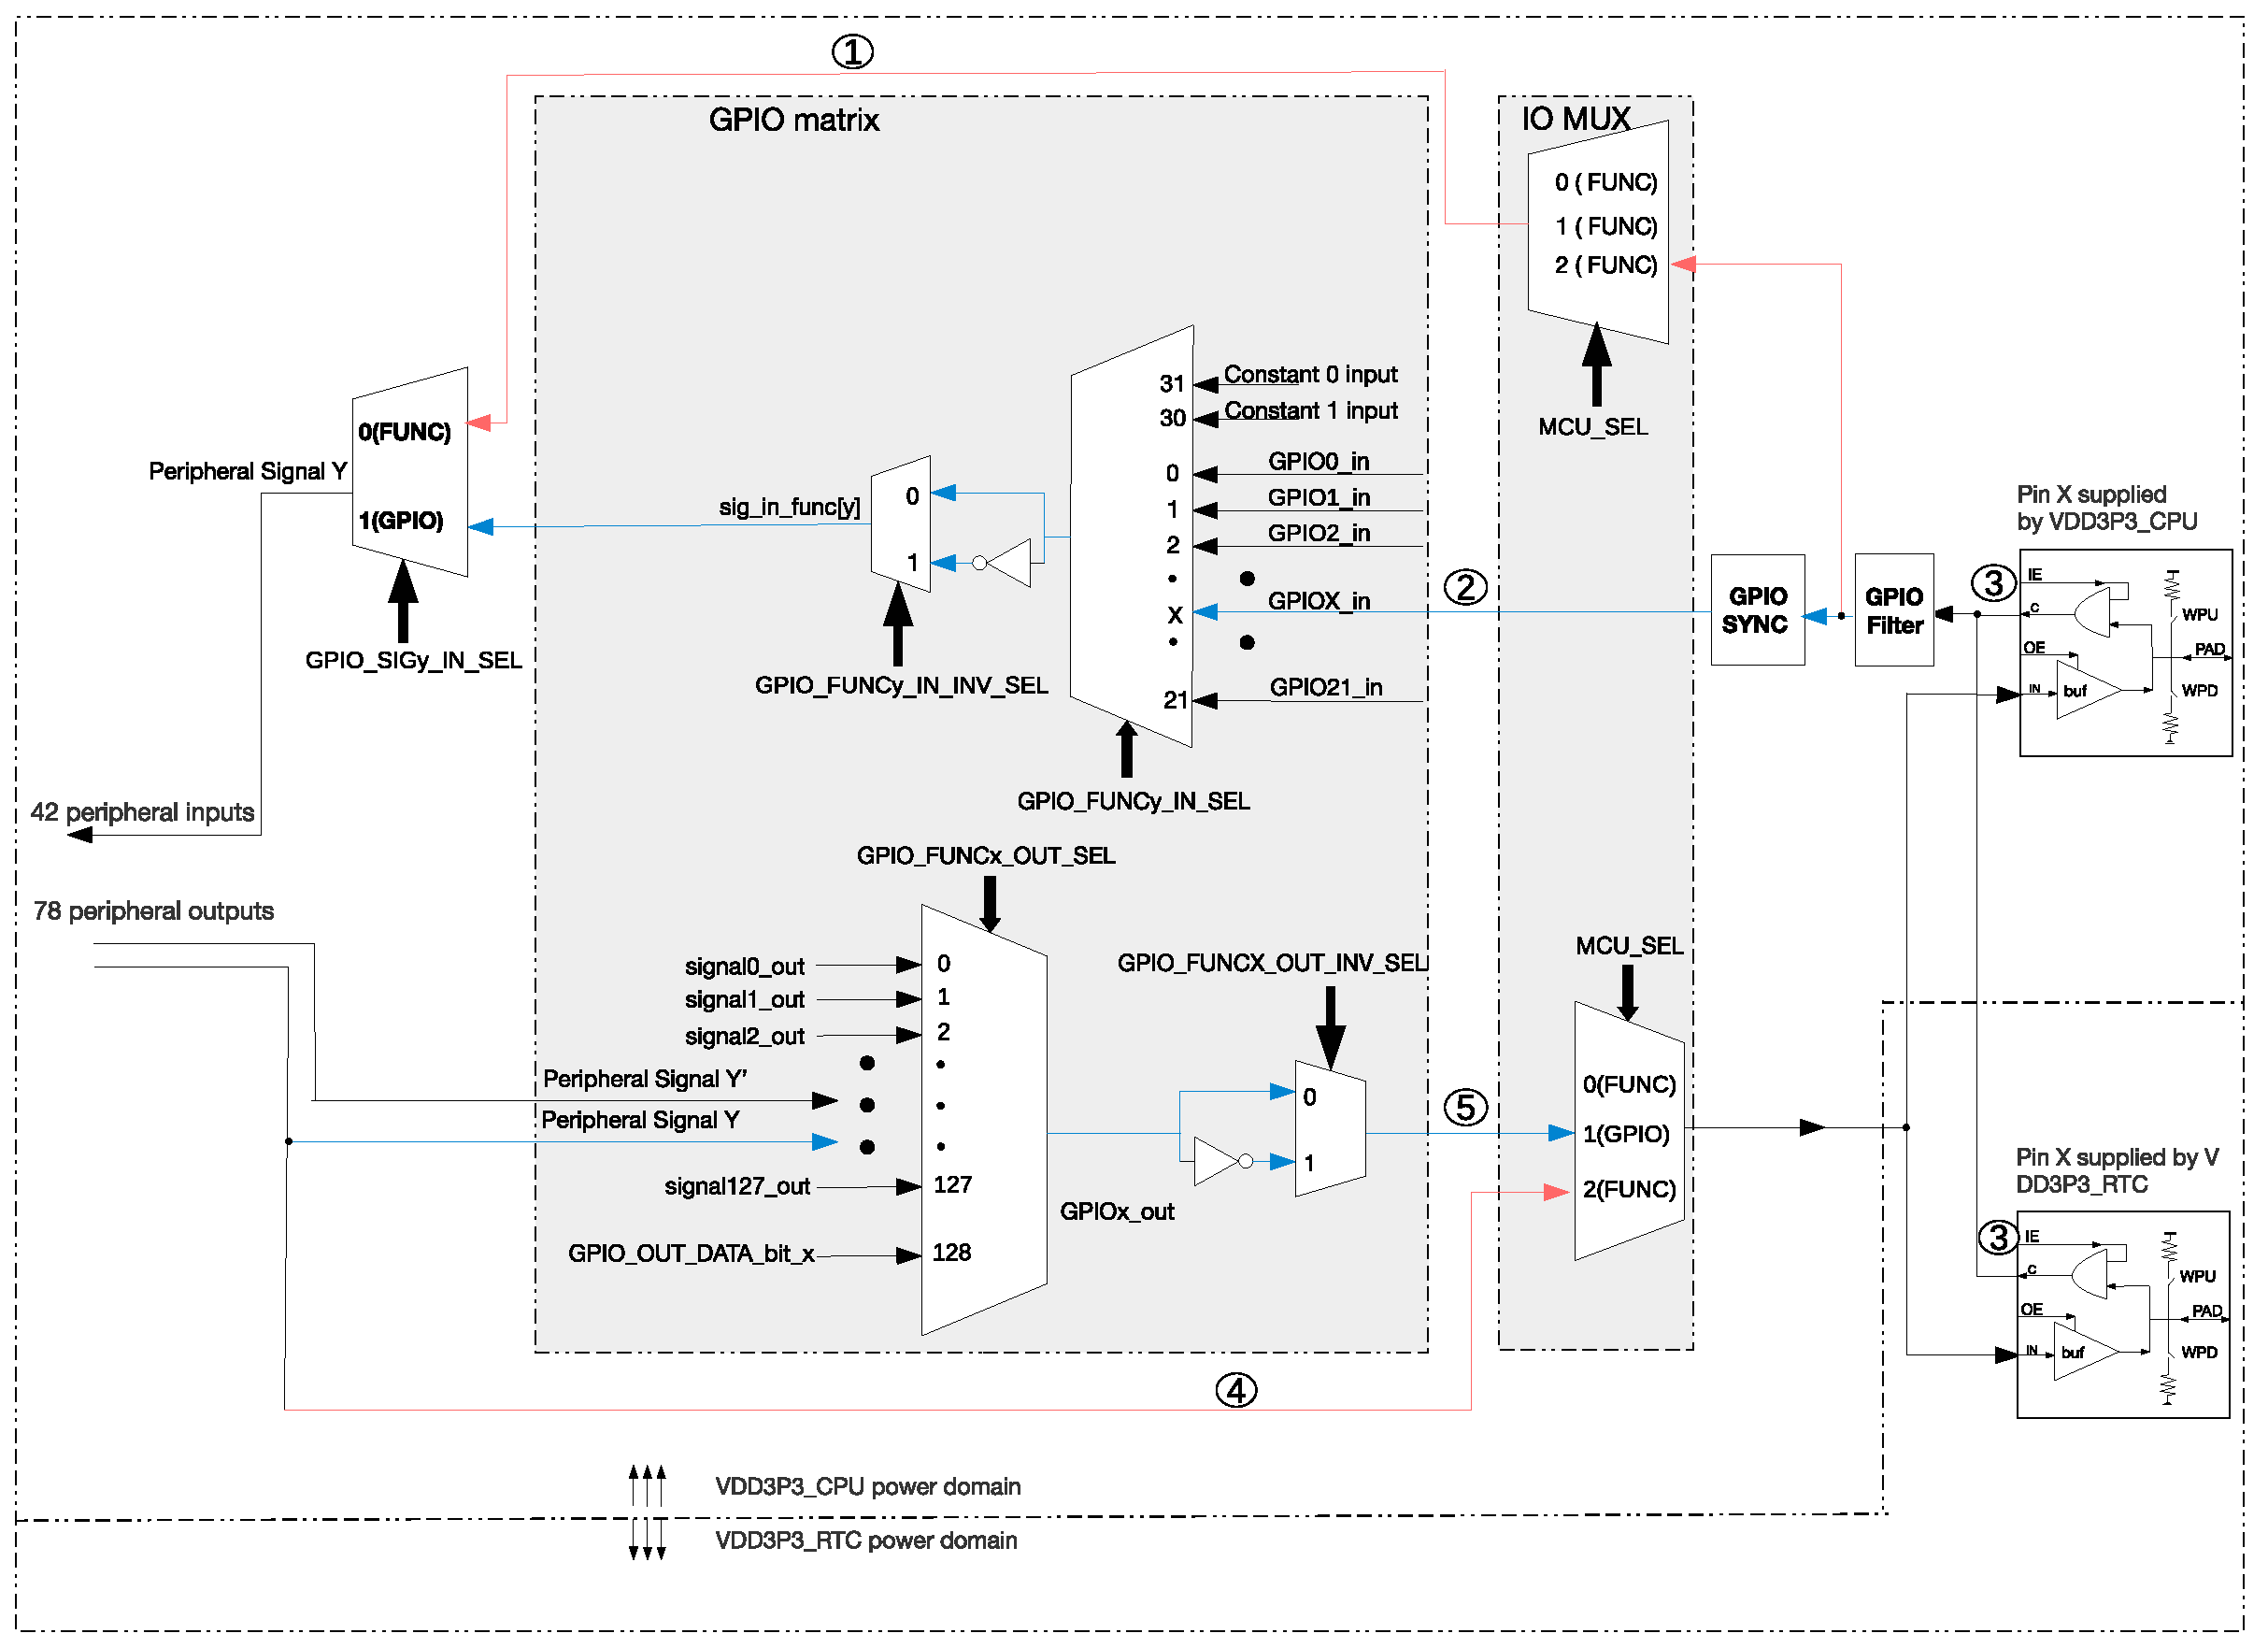
\includegraphics[width=1.0\textwidth]{16-IOMUXGPIO/figures/figure2-over-detailed-20250224}
    \caption{IO MUX 和 GPIO 交换矩阵框图（详图）}
    \label{fig:iomux-gpio-matrix-overview-detail}
\end{figure}


    \hspace{2em} \textcircled{\footnotesize 1} 仅有部分输入信号可以直接通过 IO MUX 直连外设，这些输入信号在表 \ref{tab:iomuxgpio-periph-signals-via-gpio-matrix} “信号可经由 IO MUX 直接输入”一栏中被标为 “yes”。剩余其它信号只能通过 GPIO 交换矩阵连接至外设。\\
    \hspace{2em} \textcircled{\footnotesize 2} \chipname{} 共有 22 个 GPIO 管脚，因此从 GPIO SYNC 进入到 GPIO 交换矩阵的输入共有 22 个。 \\
    \hspace{2em} \textcircled{\footnotesize 3} 位于 VDD3P3\_CPU 电源域和 VDD3P3\_RTC 电源域的管脚由 IE、OE、WPU 和 WPD 信号控制。\\
    \hspace{2em} \textcircled{\footnotesize 4} 仅有部分输出信号可通过 IO MUX 直连管脚，这些输出信号在表 \ref{tab:iomuxgpio-periph-signals-via-gpio-matrix}“信号可经由 IO MUX 直接输出”一栏中被标为 “yes”。剩余其它信号只能通过 GPIO 交换矩阵连接至外设。\\
    \hspace{2em} \textcircled{\footnotesize 5}  从 GPIO 交换矩阵到 IO MUX 的输出共有 22 个，对应 GPIO X：0 \verb+~+ 21。 \\


图 \ref{fig:pad-overview} 展示了芯片焊盘的内部结构，即芯片逻辑与 GPIO 管脚之间的电气接口。22 个 GPIO 管脚均采用这一结构，且由 IE、OE、WPU 和 WPD 信号控制。

\begin{figure}[H]
    \centering
    \fbox{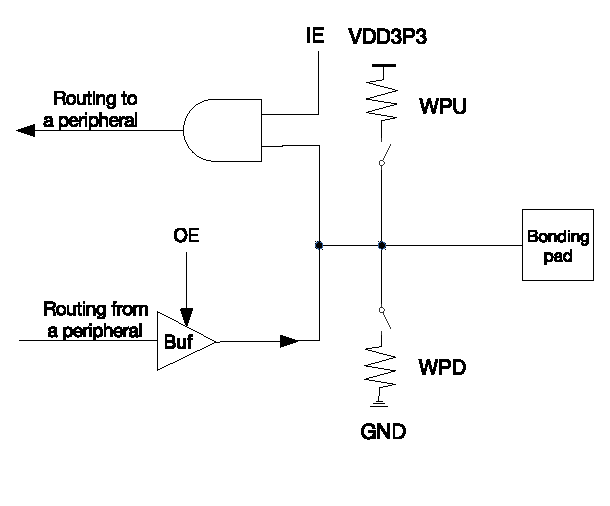
\includegraphics[width=0.6\textwidth]{16-IOMUXGPIO/figures/pad-overview_20210815.eps}}    \caption{焊盘内部结构}
    \label{fig:pad-overview}
\end{figure}

\begin{tiplisting}
\vspace{-2em}
\begin{itemize}
    \item IE：输入使能
    \item OE：输出使能
    \item WPU：内部弱上拉
    \item WPD：内部弱下拉
    \item Bonding pad：接合焊盘，芯片逻辑的结点，实现芯片封装内晶片与 GPIO 管脚之间的物理连接。
\end{itemize}
\end{tiplisting}

\section{通过 GPIO 交换矩阵的外设输入}\label{sec:peripheral-input-via-gpio-matrix}

\subsection{概述}

为实现通过 GPIO 交换矩阵接收外部输入信号，需要配置 GPIO 交换矩阵从 22 个 GPIO (0 \verb+~+ 21) 中获取外部输入信号，见交换矩阵表格 \ref{tab:iomuxgpio-periph-signals-via-gpio-matrix}。并需要配置外设输入选择通过 GPIO 交换矩阵接收输入信号。

\subsection{信号同步}
\label{sec:inputconfig}
如图 \ref{fig:iomux-gpio-matrix-overview-detail} 所示，对于信号输入，外部输入信号从 GPIO 管脚输入，经 GPIO SYNC 模块同步至 APB 总线时钟后进入 GPIO 交换矩阵。外部输入信号也可以通过 IO MUX 直接进入外设，但信号无法经由 GPIO SYNC 模块同步。


\begin{figure}[H]
    \centering
    \fbox{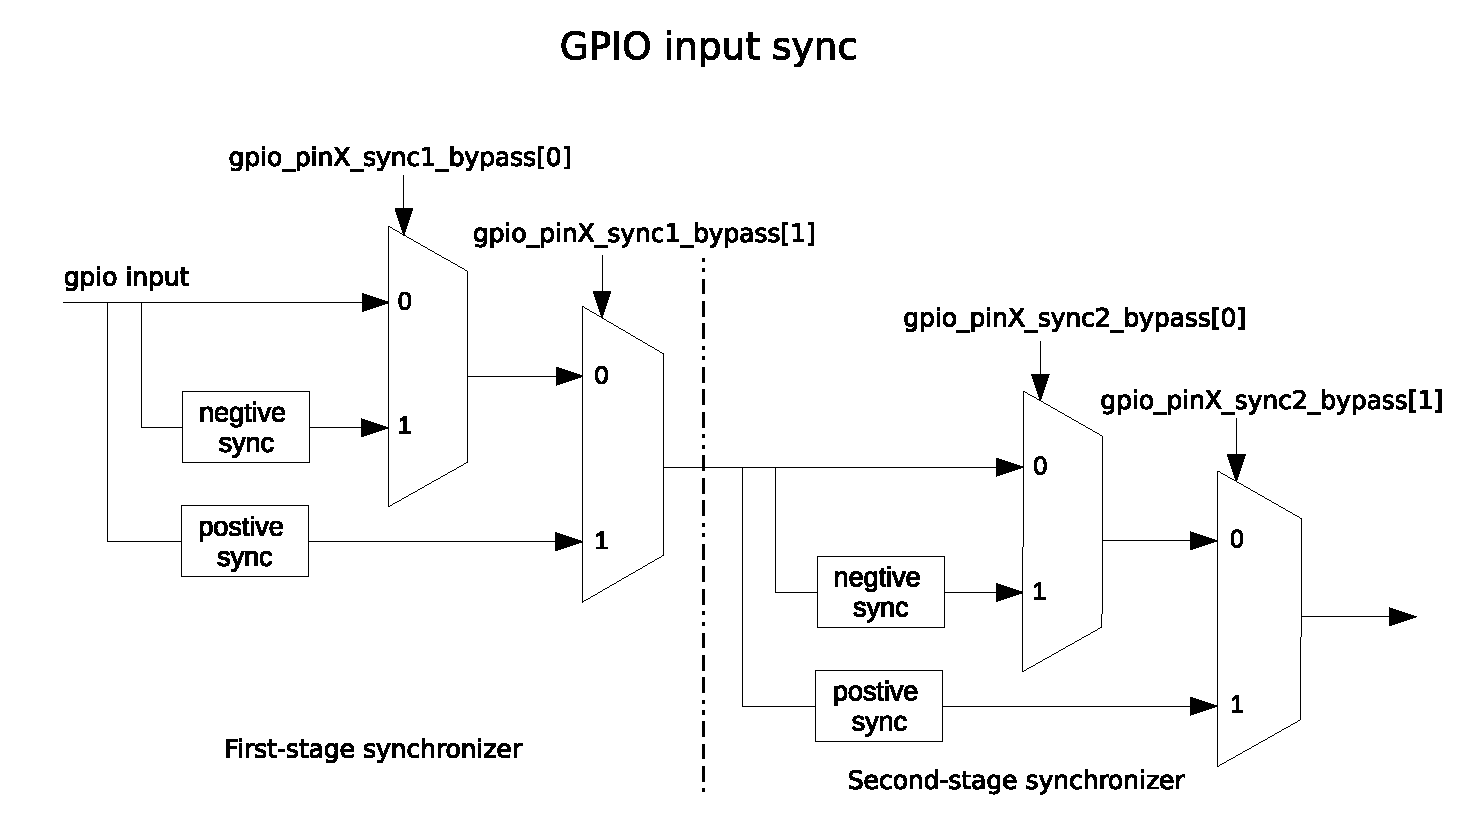
\includegraphics[width=0.7\textwidth]{16-IOMUXGPIO/figures/gpio_input_sync}}
    \caption{GPIO 输入经 APB 时钟上升沿或下降沿同步}
    \label{Figure:gpio_input_sync}
\end{figure}

GPIO SYNC 模块的功能如图 \ref{Figure:gpio_input_sync} 所示。其中，negative sync 为 GPIO 输入经过 APB 时钟的下降沿同步，positive sync 为 GPIO 输入经过 APB 时钟上升沿同步。

\subsection{功能描述}

把某个外设输入信号  \regindex{Y} 绑定到某个 GPIO 管脚  \regindex{X}\hyperref[input-note-1]{$^1$} 的配置过程如下：

\begin{enumerate}
    \item 在 GPIO 交换矩阵中配置外设信号  \regindex{Y} 的 \hyperref[regdesc:GPIOFUNCNINSELCFGREG]{GPIO\_FUNC\regindex{y}\_IN\_SEL\_CFG\_REG} 寄存器：
    \begin{itemize}
        \item 置位 \hyperref[fielddesc:GPIOSIGNINSEL]{GPIO\_SIG\regindex{y}\_IN\_SEL} 选择通过 GPIO 交换矩阵接收外部输入信号。
        \item 设置 \hyperref[fielddesc:GPIOFUNCNINSEL]{GPIO\_FUNC\regindex{y}\_IN\_SEL} 为需要的 GPIO 管脚编号，此处应为  \regindex{X}。        
    \end{itemize}
    {\bfseries 注意：}并不是所有外设信号都有有效的 \hyperref[fielddesc:GPIOSIGNINSEL]{GPIO\_SIG\regindex{y}\_IN\_SEL} 位，即有些外设信号只能通过 GPIO 交换矩阵接收外部输入信号。
    \item 可选：置位 \hyperref[fielddesc:IOMUXGPIONFILTEREN]{IO\_MUX\_GPIO\regindex{n}\_FILTER\_EN} 使能 GPIO 管脚的输入信号滤波功能，如图 \ref{Figure:gpio_filter} 所示。只有当输入信号的有效宽度大于两个时钟周期时，输入信号才会被采样。否则，输入信号将会被滤掉。
\begin{figure}[H]
    \centering
    \fbox{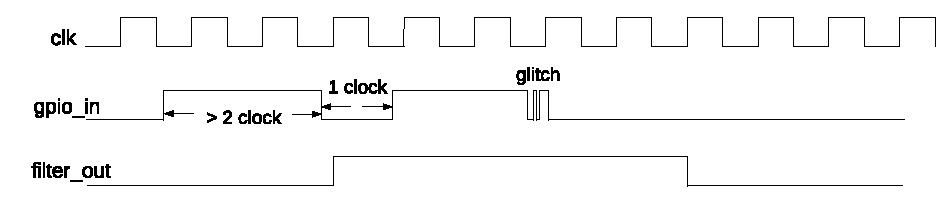
\includegraphics[width=0.9\textwidth]{16-IOMUXGPIO/figures/gpio_filter}}
    \caption{GPIO 输入信号滤波时序图}
    \label{Figure:gpio_filter}
\end{figure}

    \item 同步 GPIO 输入信号。配置 GPIO 管脚 \regindex{X} 的 \hyperref[regdesc:GPIOPINNREG]{GPIO\_PIN\regindex{x}\_REG} 来同步 GPIO 输入信号，过程如下：
    \begin{itemize}
        \item 如图 \ref{Figure:gpio_input_sync} 所示，配置 \hyperref[fielddesc:GPIOPINNSYNC1BYPASS]{GPIO\_PIN\regindex{x}\_SYNC1\_BYPASS} 使能输入信号第一拍为上升沿或下降沿同步。
        \item 如图 \ref{Figure:gpio_input_sync} 所示，配置 \hyperref[fielddesc:GPIOPINNSYNC2BYPASS]{GPIO\_PIN\regindex{x}\_SYNC2\_BYPASS} 使能输入信号第二拍为上升沿或下降沿同步。
    \end{itemize}
    \item 配置 IO MUX 寄存器使能 GPIO 管脚的输入功能。配置 GPIO 管脚 \regindex{X} 的 \hyperref[regdesc:IOMUXGPIONREG]{IO\_MUX\_GPIO\regindex{x}\_REG}，过程如下：
    \begin{itemize}
        \item 置位 \hyperref[fielddesc:IOMUXGPIONFUNIE]{IO\_MUX\_GPIO\regindex{x}\_FUN\_IE} 使能输入\hyperref[input-note-2]{$^2$}。
        \item 置位或清零 \hyperref[fielddesc:IOMUXGPIONFUNWPU]{IO\_MUX\_GPIO\regindex{x}\_FUN\_WPU} 和 \hyperref[fielddesc:IOMUXGPIONFUNWPD]{IO\_MUX\_GPIO\regindex{x}\_FUN\_WPD}，使能或关闭内部上拉/下拉电阻。
    \end{itemize}
\end{enumerate}

例如，要把 I2S MCLK 输入信号 \hyperref[input-note-3]{$^3$}（I2S\_MCLK\_in，信号索引号 12）绑定到 GPIO7，请按照以下步骤操作。注意，GPIO7 也叫做 MTDO 管脚。

\begin{enumerate}
\item 置位 \hyperref[regdesc:GPIOFUNCNINSELCFGREG]{GPIO\_FUNC12\_IN\_SEL\_CFG\_REG} 寄存器的 \hyperref[fielddesc:GPIOSIGNINSEL]{GPIO\_SIG12\_IN\_SEL} 位，使能通过 GPIO 交换矩阵接收外部输入信号；
\item 配置 \hyperref[regdesc:GPIOFUNCNINSELCFGREG]{GPIO\_FUNC12\_IN\_SEL\_CFG\_REG} 寄存器中的 \hyperref[fielddesc:GPIOFUNCNINSEL]{GPIO\_FUNC12\_IN\_SEL} 为 7，即选择管脚 GPIO7；
\item 置位 \hyperref[regdesc:IOMUXGPIONREG]{IO\_MUX\_GPIO7\_REG} 寄存器中 \hyperref[fielddesc:IOMUXGPIONFUNIE]{IO\_MUX\_GPIO7\_FUN\_IE} 位使能管脚输入。
\end{enumerate}

\begin{tiplisting}
\vspace{-2em}
\begin{enumerate}
\item \label{input-note-1} 同一个输入管脚可以同时绑定多个输入信号；
\item \label{input-note-2} 置位 \hyperref[fielddesc:GPIOFUNCNININVSEL]{GPIO\_FUNC\regindex{y}\_IN\_INV\_SEL} 可以把输入信号取反；
\item \label{input-note-3}无需将输入信号绑定到一个 GPIO 管脚也可以使外设读取恒低或恒高电平的输入值。实现方式为选择特定的 \hyperref[fielddesc:GPIOFUNCNINSEL]{GPIO\_FUNC\regindex{y}\_IN\_SEL} 输入值而不是一个 GPIO 序号：
\begin {itemize}
\item 设置 \hyperref[fielddesc:GPIOFUNCNINSEL]{GPIO\_FUNC\regindex{y}\_IN\_SEL} 为 0x1F，则输入信号恒为 0；
\item 设置 \hyperref[fielddesc:GPIOFUNCNINSEL]{GPIO\_FUNC\regindex{y}\_IN\_SEL} 为 0x1E，则输入信号恒为 1。
\end{itemize}
\end{enumerate}
\end{tiplisting}

\subsection{简单 GPIO 输入}\label{IOMUXSimpleGPIOInput}

\hyperref[regdesc:GPIOINREG]{GPIO\_IN\_REG} 寄存器存储着每个 GPIO 管脚的输入值。任意 GPIO 管脚的输入值都可以随时读取而无需为某一个外设信号配置 GPIO 交换矩阵。但需要配置 GPIO 管脚 \regindex{X} 对应的 \hyperref[regdesc:IOMUXGPIONREG]{IO\_MUX\_GPIO\regindex{x}\_REG} 中 \hyperref[fielddesc:IOMUXGPIONFUNIE]{IO\_MUX\_GPIO\regindex{x}\_FUN\\\_IE} 位以使能输入，如章节 \ref{sec:inputconfig} 所述。

\section{通过 GPIO 交换矩阵的外设输出}\label{sec:peripheral-output-via-gpio-matrix}

\subsection{概述}

为实现通过 GPIO 交换矩阵输出外设信号，需要配置 GPIO 交换矩阵将外设信号（即在表 \ref{tab:iomuxgpio-periph-signals-via-gpio-matrix} 中“输出信号”一栏所列出的信号）输出到 22 个 GPIO (0 \verb+~+ 21) 管脚。

输出信号从外设输出到 GPIO 交换矩阵，然后到达 IO MUX。IO MUX 必须设置相应管脚为 GPIO 功能，这样输出 GPIO 信号就能连接到相应管脚。

\begin{tiplisting}
表 \ref{tab:iomuxgpio-periph-signals-via-gpio-matrix} 中输出索引号为 97 \verb+~+ 100 的外设信号，没有连接至外设，可配置为从一个 GPIO 管脚输出后，直接由另一个 GPIO 管脚输入（索引号：97 \verb+~+ 100）。
\end{tiplisting}
\vspace{-2em}
\subsection{功能描述}\label{IOMUXPeripheralOutput}

如图 \ref{fig:iomux-gpio-matrix-overview-detail} 所示，对于信号输出，78 个输出信号（即在表 \ref{tab:iomuxgpio-periph-signals-via-gpio-matrix} 中“输出信号”列的所有信号）中的某一个信号通过 GPIO 交换矩阵到达 IO MUX，然后连接到某个 GPIO 管脚。

输出外设信号 \regindex{Y} 到某一 GPIO 管脚 \regindex{X}\hyperref[output-note-1]{$^1$} 的步骤如下：

\begin{enumerate}
    \item 在 GPIO 交换矩阵中配置 GPIO 管脚 \regindex{X} 的 \hyperref[regdesc:GPIOFUNCNOUTSELCFGREG]{GPIO\_FUNC\regindex{x}\_OUT\_SEL\_CFG\_REG} 寄存器和 \hyperref[regdesc:GPIOENABLEREG]{GPIO\_ENABLE\_\\REG}[\regindex{x}] 字段。推荐使用相应 \hyperref[regdesc:GPIOENABLEW1TSREG]{W1TS}（写 1 置位） 和 \hyperref[regdesc:GPIOENABLEW1TCREG]{W1TC}（写 1 清零）寄存器来更新 \hyperref[regdesc:GPIOENABLEREG]{GPIO\_ENABLE\_REG} 寄存器中的值： 
    \begin{itemize}
        \item 设置 \hyperref[regdesc:GPIOFUNCNOUTSELCFGREG]{GPIO\_FUNC\regindex{x}\_OUT\_SEL\_CFG\_REG} 寄存器的 \hyperref[fielddesc:GPIOFUNCNOUTSEL]{GPIO\_FUNC\regindex{x}\_OUT\_SEL} 字段为外设输出信号 Y 的索引号 (Y)。
        \item 要将信号强制使能为输出模式，需要将 GPIO 管脚  \regindex{X} 对应的 \hyperref[regdesc:GPIOFUNCNOUTSELCFGREG]{GPIO\_FUNC\regindex{x}\_OUT\_SEL\_CFG\_REG} 寄存器中 \hyperref[fielddesc:GPIOFUNCNOENSEL]{GPIO\_FUNC\regindex{x}\_OEN\_SEL} 字段置位；同时需要将 \hyperref[regdesc:GPIOENABLEW1TSREG]{GPIO\_ENABLE\_W1TS\_REG} 中的相应位置位。或者，将 \hyperref[fielddesc:GPIOFUNCNOENSEL]{GPIO\_FUNC\regindex{x}\_OEN\_SEL} 清零，即选择采用外设的输出使能信号，此时输出使能信号由内部逻辑功能决定。比如，表 \ref{tab:iomuxgpio-periph-signals-via-gpio-matrix} 中 ``\hyperref[fielddesc:GPIOFUNCNOENSEL]{GPIO\_FUNC\regindex{n}\_OEN\_SEL} = 0 时输出信号的输出使能信号" 一栏的 SPIQ\_oe 信号。
       \item 置位 \hyperref[regdesc:GPIOENABLEW1TCREG]{GPIO\_ENABLE\_W1TC\_REG} 中相应位可以关闭 GPIO 管脚的输出。
    \end{itemize}
    \item 要选择以开漏方式输出，可以设置 GPIO 管脚 \regindex{X} 的 \hyperref[regdesc:GPIOPINNREG]{GPIO\_PIN\regindex{x}\_REG} 寄存器中 \hyperref[fielddesc:GPIOPINNPADDRIVER]{GPIO\_PIN\regindex{x}\_PAD\_DRIVER} 位。
    \item 配置 IO MUX 寄存器来选择经由 GPIO 交换矩阵输出信号。配置 GPIO 管脚 \regindex{X} 的 \hyperref[regdesc:IOMUXGPIONREG]{IO\_MUX\_GPIO\regindex{x}\_REG} 的过程如下：
    \begin{itemize}
        \item 配置 GPIO 管脚 \regindex {X} 的 \hyperref[fielddesc:IOMUXGPIONMCUSEL]{IO\_MUX\_GPIO\regindex{x}\_MCU\_SEL} 为所需的管脚功能。此处选择数值 1，即 Function 1（GPIO 功能），适用于所有管脚。
        \item 设置 \hyperref[fielddesc:IOMUXGPIONFUNDRV]{IO\_MUX\_GPIO\regindex{x}\_FUN\_DRV} 字段为特定的输出强度值 (0 \verb+~+ 3)。
        \item 在开漏模式下，通过置位/清零 \hyperref[fielddesc:IOMUXGPIONFUNWPU]{IO\_MUX\_GPIO\regindex{x}\_FUN\_WPU} 和 \hyperref[fielddesc:IOMUXGPIONFUNWPD]{IO\_MUX\_GPIO\regindex{x}\_FUN\_WPD} 使能或关闭上拉/下拉电阻。
    \end{itemize}
\end{enumerate}

\begin{tiplisting}
\vspace{-2em}
\begin{enumerate}
\item \label{output-note-1} 某一个外设的输出信号可以同时从多个管脚输出；
\item \label{output-note-2} 置位 \hyperref[fielddesc:GPIOFUNCNOUTINVSEL]{GPIO\_FUNC\regindex{x}\_OUT\_INV\_SEL} 可以把输出的信号取反。
\end{enumerate}
\end{tiplisting}

\subsection{简单 GPIO 输出}

GPIO 交换矩阵也可用于简单 GPIO 输出，具体配置如下：

\begin{itemize}
    \item 设置 GPIO 交换矩阵 \hyperref[fielddesc:GPIOFUNCNOUTSEL]{GPIO\_FUNC\regindex{n}\_OUT\_SEL} 寄存器为特定的外设索引值 128 (0x80)；
    \item 设置 \hyperref[regdesc:GPIOOUTREG]{GPIO\_OUT\_REG} 寄存器中相应位的值为期望 GPIO 输出的值。
\end{itemize}

\begin{tiplisting}
\vspace{-2em}
\begin{itemize} 
\item \hyperref[regdesc:GPIOOUTREG]{GPIO\_OUT\_REG}[0] \verb+~+ \hyperref[regdesc:GPIOOUTREG]{GPIO\_OUT\_REG}[21] 对应 GPIO0 \verb+~+ GPIO21， \hyperref[regdesc:GPIOOUTREG]{GPIO\_OUT\_REG}[25:22] 无效。
\item 推荐使用相应的 W1TS 和 W1TC 寄存器，例如 \hyperref[fielddesc:GPIOOUTW1TS]{GPIO\_OUT\_W1TS}/\hyperref[fielddesc:GPIOOUTW1TC]{GPIO\_OUT\_W1TC} 来置位/清零 \hyperref[regdesc:GPIOOUTREG]{GPIO\_OUT\_REG}。
\end{itemize}
\end{tiplisting}

\subsection{Sigma Delta 调制输出 (SDM)}

\subsubsection{功能描述}

125 个外设输出信号中有四个信号（在表 \ref{tab:iomuxgpio-periph-signals-via-gpio-matrix} 中索引为：55 \verb+~+ 58）支持 1-bit 二阶 SDM 调制输出。上述四个信号通道默认输出使能。Sigma Delta 调制器可实现输出可配占空比的 PDM（脉冲密度调制）信号。二阶 SDM 调制的转换公式如下：

\[
    H(z)=\textrm{X(z)z$^{-1}$} + \textrm{E(z)(1-z$^{-1}$)$^{2}$}
    \]

E(z) 为量化误差，X(z) 为输入。\\
Sigma Delta 调制器内部支持对 APB\_CLK 的 1 \verb+~+ 256 倍分频： 
\begin{itemize}
    \item 置位 \hyperref[fielddesc:GPIOSDFUNCTIONCLKEN]{GPIOSD\_FUNCTION\_CLK\_EN} 使能调制器时钟；
    \item 配置 \hyperref[fielddesc:GPIOSDSDNPRESCALE]{GPIOSD\_SD\regindex{n}\_PRESCALE} 实现分频。\regindex{n} 取值范围为 0 \verb+~+ 3，对应四个信号通道。
\end{itemize}

分频后的时钟周期为调制器输出单位脉冲的周期。

\hyperref[fielddesc:GPIOSDSDNIN]{GPIOSD\_SD\regindex{n}\_IN} 为有符号数，范围为 [-128, 127]，配置此寄存器控制输出 PDM 信号的占空比$^{1}$。

\begin{itemize}
    \item \hyperref[fielddesc:GPIOSDSDNIN]{GPIOSD\_SD\regindex{n}\_IN} = -128，调制器输出信号占空比为 \begin{math}0\% \end{math}；
    \item \hyperref[fielddesc:GPIOSDSDNIN]{GPIOSD\_SD\regindex{n}\_IN} = 0，调制器输出信号占空比接近 \begin{math}50\% \end{math}；
    \item \hyperref[fielddesc:GPIOSDSDNIN]{GPIOSD\_SD\regindex{n}\_IN} = 127，调制器输出信号占空比接近 \begin{math}100\% \end{math}。
\end{itemize}

PDM 信号占空比计算公式为：

    \[
    Duty\_Cycle=\frac{\hyperref[fielddesc:GPIOSDSDNIN]{GPIOSD\_SD\regindex{n}\_IN} + 128} {256}
    \]
    
\begin{tiplisting}
对 PDM 信号来说，占空比是指在若干脉冲周期内（比如 256 个脉冲周期），高电平占整个统计周期的比值。
\end{tiplisting}

\subsubsection{配置方法}

SDM 的配置方法如下：

\begin{itemize}
    \item 将 SDM 输出经 GPIO 交换矩阵连接至相应管脚，见 \ref{IOMUXPeripheralOutput} 章节；
    \item 置位 \hyperref[fielddesc:GPIOSDFUNCTIONCLKEN]{GPIOSD\_FUNCTION\_CLK\_EN}，使能 SDM 时钟；
    \item 配置 \hyperref[fielddesc:GPIOSDSDNPRESCALE]{GPIOSD\_SD\regindex{n}\_PRESCALE} 寄存器设置时钟分频系数；
    \item 配置 \hyperref[fielddesc:GPIOSDSDNIN]{GPIOSD\_SD\regindex{n}\_IN} 寄存器设置 SDM 输出信号的占空比。
\end{itemize}

\section{IO MUX 的直接输入输出功能}

\subsection{概述}

快速信号如 SPI、JTAG 等会旁路 GPIO 交换矩阵以实现更好的高频数字特性。所以高速信号会直接通过 IO MUX 输入和输出。

这样比使用 GPIO 交换矩阵的灵活度要低，即每个 GPIO 管脚的 IO MUX 寄存器只有较少的功能选择，但可以实现更好的高频数字特性。

\subsection{功能描述}

对于外设输入信号，旁路 GPIO 交换矩阵必须配置两个寄存器：

\begin{enumerate}
\item GPIO 管脚的 \hyperref[fielddesc:IOMUXGPIONMCUSEL]{IO\_MUX\_GPIO\regindex{n}\_MCU\_SEL} 必须设置为相应的管脚功能，章节 \ref{sec:iomux_pads} 列出了管脚功能。
\item 清零 \hyperref[fielddesc:GPIOSIGNINSEL]{GPIO\_SIG\regindex{n}\_IN\_SEL}，直接将输入信号连接到外设。
\end{enumerate}

对于外设输出信号，旁路 GPIO 交换矩阵只需将 GPIO 管脚的 \hyperref[fielddesc:IOMUXGPIONMCUSEL]{IO\_MUX\_GPIO\regindex{n}\_MCU\_SEL} 配置为相应的管脚功能即可。

\begin{tiplisting}
并非所有外设输入/输出信号均可直接通过 IO MUX 连接到外设，某些输入/输出信号只能通过 GPIO 交换矩阵连接到外设。
\end{tiplisting}

\section{GPIO 管脚的模拟功能}

\chipname{} 部分 GPIO 管脚具有模拟功能。用于模拟功能时，请确保已按照下述方法关闭了上拉电阻和下拉电阻：

\begin{itemize}
    \item 设置 \hyperref[fielddesc:IOMUXGPIONMCUSEL]{IO\_MUX\_GPIO\regindex{n}\_MCU\_SEL} 为 1，同时清零 \hyperref[fielddesc:IOMUXGPIONFUNIE]{IO\_MUX\_GPIO\regindex{n}\_FUN\_IE}、\hyperref[fielddesc:IOMUXGPIONFUNIE]{IO\_MUX\_GPIO\regindex{n}\_FUN\_WPU}、\hyperref[fielddesc:IOMUXGPIONFUNIE]{IO\_MUX\_GPIO\regindex{n}\_FUN\_WPD}；
    \item 置位 \hyperref[fielddesc:GPIOENABLEW1TC]{GPIO\_ENABLE\_W1TC\regindex{[n]}}，清除输出使能。
\end{itemize}
表 \ref{tab:iomuxgpio-iomax-pins-analog-functions} 列出了 \chipname{} 管脚的模拟功能。

\section{Light-sleep 模式管脚功能}

当 \chipname{} 处于 Light-sleep 模式时管脚可以有不同的功能。如果某一 GPIO 管脚的 \hyperref[regdesc:IOMUXGPIONREG]{IO\_MUX\_\regindex{n}\_REG} 寄存器中 \hyperref[fielddesc:IOMUXGPIONSLPSEL]{IO\_MUX\_SLP\_SEL} 位置为 1，芯片处于 Light-sleep 模式下将由另一组不同的寄存器控制管脚。

\begin{longtable}[c]{|p{3cm}|m{6.5cm}|m{5cm}|}
\caption{IO MUX Light-sleep 管脚功能控制寄存器}
\label{tab:iomuxgpio-pin-function-register-light-sleep-mode} \\
    \hline
    \rowcolor{lightgray}
   & 正常工作模式 & Light-sleep 模式 \\
    \rowcolor{lightgray}
   \multirow{-2}{*}{IO MUX 功能}  & OR \hyperref[fielddesc:IOMUXGPIONSLPSEL]{IO\_MUX\_SLP\_SEL} = 0 & AND \hyperref[fielddesc:IOMUXGPIONSLPSEL]{IO\_MUX\_SLP\_SEL} = 1 \\
    \hline
输出驱动强度 & \hyperref[fielddesc:IOMUXGPIONFUNDRV]{IO\_MUX\_FUN\_DRV} & \hyperref[fielddesc:IOMUXGPIONMCUDRV]{IO\_MUX\_MCU\_DRV} \\ 
\hline
上拉电阻 & \hyperref[fielddesc:IOMUXGPIONFUNWPU]{IO\_MUX\_FUN\_WPU} & \hyperref[fielddesc:IOMUXGPIONMCUWPU]{IO\_MUX\_MCU\_WPU} \\
\hline
下拉电阻 & \hyperref[fielddesc:IOMUXGPIONFUNWPD]{IO\_MUX\_FUN\_WPD} & \hyperref[fielddesc:IOMUXGPIONMCUWPD]{IO\_MUX\_MCU\_WPD} \\
\hline
输出使能 & 由 GPIO 交换矩阵的 \hyperref[fielddesc:GPIOFUNCNOENSEL]{OEN\_SEL} 位控制 $^{*}$ & \hyperref[fielddesc:IOMUXGPIONMCUOE]{IO\_MUX\_MCU\_OE} \\
\hline
\end{longtable}

\begin{tiplisting}
如果 \hyperref[fielddesc:IOMUXGPIONSLPSEL]{IO\_MUX\_SLP\_SEL} 置为 0，则芯片在正常工作和 Light-sleep 模式下，管脚的功能一样。此时，具体的输出使能配置请参考 \ref{IOMUXPeripheralOutput} 章节。

\end{tiplisting}

\section{管脚 Hold 特性}\label{PadHold}

每个 GPIO 管脚（包括 RTC 管脚 GPIO0 \verb+~+ GPIO5）都有单独的 Hold 功能，由 RTC 寄存器控制。管脚的 Hold 功能被置上后，管脚在置上 Hold 那一刻的状态被强制保持，无论内部信号如何变化，修改 IO MUX 配置或者 GPIO 配置，都不会改变管脚的状态。应用如果希望在看门狗超时触发内核复位时或 Deep-sleep 触发内核复位时管脚的状态不被改变，就需要提前把 Hold 置上。

\begin{itemize}
\item \textbf{数字管脚 (GPIO6 $\sim$ GPIO21)}\\
每个数字管脚的 Hold 状态由各管脚的 Hold 使能信号和全局的 Hold 使能信号经过或运算后共同控制。
\begin{itemize}
    \item \hyperref[regdesc:RTCCNTLDIGPADHOLDREG] {RTC\_CNTL\_DIG\_PAD\_HOLD\_REG[\regindex{n}]}，控制 GPIO6 \verb+~+ GPIO21 各个管脚的 Hold 使能信号。
    \item \hyperref[fielddesc:RTCCNTLDGPADFORCEHOLD]{RTC\_CNTL\_DG\_PAD\_FORCE\_HOLD}，控制数字管脚全局的 Hold 使能信号。
\end{itemize}
要使用此功能，请按照以下步骤操作：

\begin{itemize}
    \item 若要在 Deep-sleep 中保持管脚输入输出的状态值，需要在掉电之前将寄存器 \hyperref[regdesc:RTCCNTLDIGPADHOLDREG]{RTC\_\\CNTL\_DIG\_PAD\_HOLD\_REG[\regindex{n}]} 置位。在芯片被唤醒后，若要关闭 Hold 功能，可将上述寄存器清零。
    \item 或者，将 \hyperref[fielddesc:RTCCNTLDGPADFORCEHOLD]{RTC\_CNTL\_DG\_PAD\_FORCE\_HOLD} 置位，用以保持所有数字管脚的状态值。在芯片被唤醒后，也可将 \hyperref[fielddesc:RTCCNTLDGPADFORCEUNHOLD]{RTC\_CNTL\_DG\_PAD\_FORCE\_UNHOLD} 置位，用以关闭所有数字管脚的 Hold 功能。
\end{itemize}


\item \textbf{RTC 管脚 (GPIO0 $\sim$ GPIO5)}\\
每个 RTC 管脚的 Hold 状态由各管脚的 Hold 使能信号和全局的 Hold 使能信号经过或运算后共同控制。
\begin{itemize}
    \item \hyperref[regdesc:RTCCNTLPADHOLDREG]{RTC\_CNTL\_PAD\_HOLD\_REG}[\regindex{n}](\regindex{n} = 0 \verb+~+ 5)，控制 GPIO0 \verb+~+ GPIO5 各个管脚的 Hold 使能信号。
    \item \hyperref[fielddesc:RTCCNTLRTCPADFORCEHOLD]{RTC\_CNTL\_RTC\_PAD\_FORCE\_HOLD} 控制 RTC 管脚全局的 Hold 使能信号。
\end{itemize}

要使用此功能，请按照以下步骤操作：

管脚的输入输出值由寄存器 \hyperref[regdesc:RTCCNTLPADHOLDREG]{RTC\_CNTL\_PAD\_HOLD\_REG} 中的相应位控制。用户可置位或清除相应位来实现 Hold 或 Unhold 管脚输入输出值。
\end{itemize}



\section{GPIO 管脚供电和电源管理}\label{I/O Pad Power Supplies}

\subsection{GPIO 管脚供电}
GPIO 管脚供电请参考  {\it{\href{https://www.espressif.com/sites/default/files/documentation/esp32-c3_datasheet_en.pdf}{《\chipname{} 规格书》}}} 中管脚定义章节。所有管脚均可用于将芯片从 Light-sleep 中唤醒，但仅有 VDD3P3\_RTC 域中的管脚 (GPIO0 \verb+~+ GPIO5) 可用于将芯片从 Deep-sleep 唤醒。

\subsection{电源管理}

\chipname{} 的管脚可分为如下两种不同的电源域。

\begin{itemize}
    \item VDD3P3\_RTC：RTC 和 CPU 的输入电源
    \item VDD3P3\_CPU：CPU 的输入电源
\end{itemize}

\section{外设信号列表}
\label{sec:peripheral_signals}

表 \ref{tab:iomuxgpio-periph-signals-via-gpio-matrix} 列出了所有经由 GPIO 交换矩阵的外设输入输出信号。

请注意 \hyperref[fielddesc:GPIOFUNCNOENSEL]{GPIO\_FUNC\regindex{n}\_OEN\_SEL} 位的配置：

\begin{itemize}
    \item \hyperref[fielddesc:GPIOFUNCNOENSEL]{GPIO\_FUNC\regindex{n}\_OEN\_SEL} = 1，则寄存器 \hyperref[regdesc:GPIOENABLEREG]{GPIO\_ENABLE\_REG} 中的相应位  \regindex{n} 将用于控制信号输出使能。
    \begin{itemize}
        \item \hyperref[regdesc:GPIOENABLEREG]{GPIO\_ENABLE\_REG} = 0：输出关闭；
        \item \hyperref[regdesc:GPIOENABLEREG]{GPIO\_ENABLE\_REG} = 1：输出使能；
    \end{itemize}
    \item \hyperref[fielddesc:GPIOFUNCNOENSEL]{GPIO\_FUNC\regindex{n}\_OEN\_SEL} = 0，则输出信号的使能由外设控制，例如表 \ref{tab:iomuxgpio-periph-signals-via-gpio-matrix} 中 ``\hyperref[fielddesc:GPIOFUNCNOENSEL]{GPIO\_FUNC\regindex{n}\_OEN\_SEL} = 0 时输出信号的输出使能信号" 一栏的 SPIQ\_oe。注意，使能信号 SPIQ\_oe 可设置为 1 (1'd1) 或 0 (1'd0)，具体由外设的配置决定。如果 ``\hyperref[fielddesc:GPIOFUNCNOENSEL]{GPIO\_FUNC\regindex{n}\_OEN\_SEL} = 0 时输出信号的输出使能信号" 一栏中为 1'd1，则表示寄存器 \hyperref[fielddesc:GPIOFUNCNOENSEL]{GPIO\_FUNC\regindex{n}\_OEN\_SEL} 已清零，输出信号默认始终使能。
\end{itemize}

\begin{tiplisting}
信号连续编号，但并非所有信号均有效。
\vspace{-1em}
\begin{itemize}
    \item 表 \ref{tab:iomuxgpio-periph-signals-via-gpio-matrix}“输入信号”一栏中有名字的信号均为有效输入信号；
    \item 表 \ref{tab:iomuxgpio-periph-signals-via-gpio-matrix}“输出信号”一栏中有名字的信号均为有效输出信号。
\end{itemize}
\end{tiplisting}

\begin{landscape}

\begin{longtable}{|L{1.1cm}|L{4.0cm}|C{1.2cm}|C{1.8cm}|L{4.3cm}|L{5.0cm}|C{1.8cm}| }
     \caption{GPIO 交换矩阵外设信号}
     \label{tab:iomuxgpio-periph-signals-via-gpio-matrix} \\
     \hline
     \rowcolor{lightgray}
\textbf{信号索引} & \textbf{输入信号} & \textbf{默认值} &  \textbf{信号可经由 IO MUX 直接输入} & \textbf{输出信号} & \textbf{\hyperref[fielddesc:GPIOFUNCNOENSEL]{GPIO\_FUNC\regindex{n}\_OEN\_SEL} = 0 时输出信号的输出使能信号} & \textbf{信号可经由 IO MUX 直接输出}\\
\hline
\endfirsthead
     \hline
     \rowcolor{lightgray}
\textbf{信号索引} & \textbf{输入信号} & \textbf{默认值} &  \textbf{信号可经由 IO MUX 直接输入} & \textbf{输出信号} & \textbf{\hyperref[fielddesc:GPIOFUNCNOENSEL]{GPIO\_FUNC\regindex{n}\_OEN\_SEL} = 0 时输出信号的输出使能信号} & \textbf{信号可经由 IO MUX 直接输出}\\
     \hline
     \endhead
     \endfoot
  0  &                     SPIQ\_in  &  0  &  yes  &              SPIQ\_out  &                 SPIQ\_oe &  yes   \\\hline
  1  &                     SPID\_in  &  0  &  yes  &              SPID\_out  &                 SPID\_oe &  yes   \\\hline
  2  &                    SPIHD\_in  &  0  &  yes  &             SPIHD\_out  &                SPIHD\_oe &  yes   \\\hline
  3  &                    SPIWP\_in  &  0  &  yes  &             SPIWP\_out  &                SPIWP\_oe &  yes   \\\hline
  4  &                            -  &  -  &    -  &       SPICLK\_out\_mux  &               SPICLK\_oe &  yes   \\\hline
  5  &                            -  &  -  &    -  &            SPICS0\_out  &               SPICS0\_oe &  yes   \\\hline
  6  &                    U0RXD\_in  &  0  &  yes  &             U0TXD\_out  &                     1'd1 &  yes   \\\hline
  7  &                    U0CTS\_in  &  0  &  no  &             U0RTS\_out  &                     1'd1 &   no   \\\hline
  8  &                    U0DSR\_in  &  0  &   no  &             U0DTR\_out  &                     1'd1 &   no   \\\hline
  9  &                    U1RXD\_in  &  0  &  no  &             U1TXD\_out  &                     1'd1 &   no   \\\hline
 10  &                    U1CTS\_in  &  0  &  no  &             U1RTS\_out  &                     1'd1 &   no   \\\hline
 11  &                    U1DSR\_in  &  0  &   no  &             U1DTR\_out  &                     1'd1 &   no   \\\hline
 12  &                I2S\_MCLK\_in  &  0  &   no  &         I2S\_MCLK\_out  &                     1'd1 &   no   \\\hline
 13  &                I2SO\_BCK\_in  &  0  &   no  &         I2SO\_BCK\_out  &                     1'd1 &   no   \\\hline
 14  &                 I2SO\_WS\_in  &  0  &   no  &          I2SO\_WS\_out  &                     1'd1 &   no   \\\hline
 15  &                 I2SI\_SD\_in  &  0  &   no  &          I2SO\_SD\_out  &                     1'd1 &   no   \\\hline
 16  &                I2SI\_BCK\_in  &  0  &   no  &         I2SI\_BCK\_out  &                     1'd1 &   no   \\\hline
 17  &                 I2SI\_WS\_in  &  0  &   no  &          I2SI\_WS\_out  &                     1'd1 &   no   \\\hline
 18  &           gpio\_bt\_priority  &  0  &   no  &       gpio\_wlan\_prio  &                     1'd1 &   no   \\\hline
 19  &             gpio\_bt\_active  &  0  &   no  &     gpio\_wlan\_active  &                     1'd1 &   no   \\\hline
 20  &                            -  &  -  &    -  &                      -  &                     1'd1 &   no   \\\hline
 21  &                            -  &  -  &    -  &                      -  &                     1'd1 &   no   \\\hline
 22  &                            -  &  -  &    -  &                      -  &                     1'd1 &   no   \\\hline
 23  &                            -  &  -  &    -  &                      -  &                     1'd1 &   no   \\\hline
 24  &                            -  &  -  &    -  &                      -  &                     1'd1 &   no   \\\hline
 25  &                            -  &  -  &    -  &                      -  &                     1'd1 &   no   \\\hline
 26  &                            -  &  -  &    -  &                      -  &                     1'd1 &   no   \\\hline
 27  &                            -  &  -  &    -  &                      -  &                     1'd1 &   no   \\\hline
 28  &               cpu\_gpio\_in0  &  0  &   no  &        cpu\_gpio\_out0  &     cpu\_gpio\_out\_oen0 &   no   \\\hline
 29  &               cpu\_gpio\_in1  &  0  &   no  &        cpu\_gpio\_out1  &     cpu\_gpio\_out\_oen1 &   no   \\\hline
 30  &               cpu\_gpio\_in2  &  0  &   no  &        cpu\_gpio\_out2  &     cpu\_gpio\_out\_oen2 &   no   \\\hline
 31  &               cpu\_gpio\_in3  &  0  &   no  &        cpu\_gpio\_out3  &     cpu\_gpio\_out\_oen3 &   no   \\\hline
 32  &               cpu\_gpio\_in4  &  0  &   no  &        cpu\_gpio\_out4  &     cpu\_gpio\_out\_oen4 &   no   \\\hline
 33  &               cpu\_gpio\_in5  &  0  &   no  &        cpu\_gpio\_out5  &     cpu\_gpio\_out\_oen5 &   no   \\\hline
 34  &               cpu\_gpio\_in6  &  0  &   no  &        cpu\_gpio\_out6  &     cpu\_gpio\_out\_oen6 &   no   \\\hline
 35  &               cpu\_gpio\_in7  &  0  &   no  &        cpu\_gpio\_out7  &     cpu\_gpio\_out\_oen7 &   no   \\\hline
 36  &                            -  &  -  &    -  &         usb\_jtag\_tck  &                     1'd1 &   no   \\\hline
 37  &                            -  &  -  &    -  &         usb\_jtag\_tms  &                     1'd1 &   no   \\\hline
 38  &                            -  &  -  &    -  &         usb\_jtag\_tdi  &                     1'd1 &   no   \\\hline
 39  &                            -  &  -  &    -  &         usb\_jtag\_tdo  &                     1'd1 &   no   \\\hline
 40  &                            -  &  -  &    -  &                      -  &                     1'd1 &   no   \\\hline
 41  &                            -  &  -  &    -  &                      -  &                     1'd1 &   no   \\\hline
 42  &                            -  &  -  &    -  &                      -  &                     1'd1 &   no   \\\hline
 43  &                            -  &  -  &    -  &                      -  &                     1'd1 &   no   \\\hline
 44  &                            -  &  -  &    -  &                      -  &                     1'd1 &   no   \\\hline
 45  &              ext\_adc\_start  &  0  &   no  &    ledc\_ls\_sig\_out0  &                     1'd1 &   no   \\\hline
 46  &                            -  &  -  &    -  &    ledc\_ls\_sig\_out1  &                     1'd1 &   no   \\\hline
 47  &                            -  &  -  &    -  &    ledc\_ls\_sig\_out2  &                     1'd1 &   no   \\\hline
 48  &                            -  &  -  &    -  &    ledc\_ls\_sig\_out3  &                     1'd1 &   no   \\\hline
 49  &                            -  &  -  &    -  &    ledc\_ls\_sig\_out4  &                     1'd1 &   no   \\\hline
 50  &                            -  &  -  &    -  &    ledc\_ls\_sig\_out5  &                     1'd1 &   no   \\\hline
 51  &              rmt\_sig\_in0    &  0  &   no  &         rmt\_sig\_out0  &                     1'd1 &   no   \\\hline
 52  &              rmt\_sig\_in1    &  0  &   no  &         rmt\_sig\_out1  &                     1'd1 &   no   \\\hline
 53  &             I2CEXT0\_SCL\_in  &  1  &   no  &      I2CEXT0\_SCL\_out  &         I2CEXT0\_SCL\_oe &   no   \\\hline
 54  &             I2CEXT0\_SDA\_in  &  1  &   no  &      I2CEXT0\_SDA\_out  &         I2CEXT0\_SDA\_oe &   no   \\\hline
 55  &                            -  &  -  &    -  &         gpio\_sd0\_out  &                     1'd1 &   no   \\\hline
 56  &                            -  &  -  &    -  &         gpio\_sd1\_out  &                     1'd1 &   no   \\\hline
 57  &                            -  &  -  &    -  &         gpio\_sd2\_out  &                     1'd1 &   no   \\\hline
 58  &                            -  &  -  &    -  &         gpio\_sd3\_out  &                     1'd1 &   no   \\\hline
 59  &                            -  &  -  &    -  &         I2SO\_SD1\_out  &                     1'd1 &   no   \\\hline
 60  &                            -  &  -  &    -  &                      -  &                     1'd1 &   no   \\\hline
 61  &                            -  &  -  &    -  &                      -  &                     1'd1 &   no   \\\hline
 62  &                            -  &  -  &    -  &                      -  &                     1'd1 &   no   \\\hline
 63  &                  FSPICLK\_in  &  0  &  yes  &      FSPICLK\_out\_mux  &              FSPICLK\_oe &  yes   \\\hline
 64  &                    FSPIQ\_in  &  0  &  yes  &             FSPIQ\_out  &                FSPIQ\_oe &  yes   \\\hline
 65  &                    FSPID\_in  &  0  &  yes  &             FSPID\_out  &                FSPID\_oe &  yes   \\\hline
 66  &                   FSPIHD\_in  &  0  &  yes  &            FSPIHD\_out  &               FSPIHD\_oe &  yes   \\\hline
 67  &                   FSPIWP\_in  &  0  &  yes  &            FSPIWP\_out  &               FSPIWP\_oe &  yes   \\\hline
 68  &                  FSPICS0\_in  &  0  &  yes  &           FSPICS0\_out  &              FSPICS0\_oe &  yes   \\\hline
 69  &                            -  &  -  &    -  &           FSPICS1\_out  &              FSPICS1\_oe &   no   \\\hline
 70  &                            -  &  -  &    -  &           FSPICS2\_out  &              FSPICS2\_oe &   no   \\\hline
 71  &                            -  &  -  &    -  &           FSPICS3\_out  &              FSPICS3\_oe &   no   \\\hline
 72  &                            -  &  -  &    -  &           FSPICS4\_out  &              FSPICS4\_oe &   no   \\\hline
 73  &                            -  &  -  &    -  &           FSPICS5\_out  &              FSPICS5\_oe &   no   \\\hline
 74  &                     twai\_rx  &  1  &   no  &               twai\_tx  &                     1'd1 &   no   \\\hline
 75  &                            -  &  -  &    -  &     twai\_bus\_off\_on  &                     1'd1 &   no   \\\hline
 76  &                            -  &  -  &    -  &           twai\_clkout  &                     1'd1 &   no   \\\hline
 77  &                            -  &  -  &    -  &                      -  &                     1'd1 &   no   \\\hline
 78  &                            -  &  -  &    -  &                      -  &                     1'd1 &   no   \\\hline
 79  &                            -  &  -  &    -  &                      -  &                     1'd1 &   no   \\\hline
 80  &                            -  &  -  &    -  &                      -  &                     1'd1 &   no   \\\hline
 81  &                            -  &  -  &    -  &                      -  &                     1'd1 &   no   \\\hline
 82  &                            -  &  -  &    -  &                      -  &                     1'd1 &   no   \\\hline
 83  &                            -  &  -  &    -  &                      -  &                     1'd1 &   no   \\\hline
 84  &                            -  &  -  &    -  &                      -  &                     1'd1 &   no   \\\hline
 85  &                            -  &  -  &    -  &                      -  &                     1'd1 &   no   \\\hline
 86  &                            -  &  -  &    -  &                      -  &                     1'd1 &   no   \\\hline
 87  &                            -  &  -  &    -  &                      -  &                     1'd1 &   no   \\\hline
 88  &                            -  &  -  &    -  &                      -  &                     1'd1 &   no   \\\hline
 89  &                            -  &  -  &    -  &              ant\_sel0  &                     1'd1 &   no   \\\hline
 90  &                            -  &  -  &    -  &              ant\_sel1  &                     1'd1 &   no   \\\hline
 91  &                            -  &  -  &    -  &              ant\_sel2  &                     1'd1 &   no   \\\hline
 92  &                            -  &  -  &    -  &              ant\_sel3  &                     1'd1 &   no   \\\hline
 93  &                            -  &  -  &    -  &              ant\_sel4  &                     1'd1 &   no   \\\hline
 94  &                            -  &  -  &    -  &              ant\_sel5  &                     1'd1 &   no   \\\hline
 95  &                            -  &  -  &    -  &              ant\_sel6  &                     1'd1 &   no   \\\hline
 96  &                            -  &  -  &    -  &              ant\_sel7  &                     1'd1 &   no   \\\hline
 97  &            sig\_in\_func\_97  &  0  &   no  &        sig\_in\_func97  &                     1'd1 &   no   \\\hline
 98  &            sig\_in\_func\_98  &  0  &   no  &        sig\_in\_func98  &                     1'd1 &   no   \\\hline
 99  &            sig\_in\_func\_99  &  0  &   no  &        sig\_in\_func99  &                     1'd1 &   no   \\\hline
100  &           sig\_in\_func\_100  &  0  &   no  &       sig\_in\_func100  &                     1'd1 &   no   \\\hline
101  &                            -  &  -  &    -  &                      -  &                     1'd1 &   no   \\\hline
102  &                            -  &  -  &    -  &                      -  &                     1'd1 &   no   \\\hline
103  &                            -  &  -  &    -  &                      -  &                     1'd1 &   no   \\\hline
104  &                            -  &  -  &    -  &                      -  &                     1'd1 &   no   \\\hline
105  &                            -  &  -  &    -  &                      -  &                     1'd1 &   no   \\\hline
106  &                            -  &  -  &    -  &                      -  &                     1'd1 &   no   \\\hline
107  &                            -  &  -  &    -  &                      -  &                     1'd1 &   no   \\\hline
108  &                            -  &  -  &    -  &                      -  &                     1'd1 &   no   \\\hline
109  &                            -  &  -  &    -  &                      -  &                     1'd1 &   no   \\\hline
110  &                            -  &  -  &    -  &                      -  &                     1'd1 &   no   \\\hline
111  &                            -  &  -  &    -  &                      -  &                     1'd1 &   no   \\\hline
112  &                            -  &  -  &    -  &                      -  &                     1'd1 &   no   \\\hline
113  &                            -  &  -  &    -  &                      -  &                     1'd1 &   no   \\\hline
114  &                            -  &  -  &    -  &                      -  &                     1'd1 &   no   \\\hline
115  &                            -  &  -  &    -  &                      -  &                     1'd1 &   no   \\\hline
116  &                            -  &  -  &    -  &                      -  &                     1'd1 &   no   \\\hline
117  &                            -  &  -  &    -  &                      -  &                     1'd1 &   no   \\\hline
118  &                            -  &  -  &    -  &                      -  &                     1'd1 &   no   \\\hline
119  &                            -  &  -  &    -  &                      -  &                     1'd1 &   no   \\\hline
120  &                            -  &  -  &    -  &                      -  &                     1'd1 &   no   \\\hline
121  &                            -  &  -  &    -  &                      -  &                     1'd1 &   no   \\\hline
122  &                            -  &  -  &    -  &                      -  &                     1'd1 &   no   \\\hline
123  &                            -  &  -  &    -  &         CLK\_OUT\_out1  &                     1'd1 &   no   \\\hline
124  &                            -  &  -  &    -  &         CLK\_OUT\_out2  &                     1'd1 &   no   \\\hline
125  &                            -  &  -  &    -  &         CLK\_OUT\_out3  &                     1'd1 &   no   \\\hline
126  &                            -  &  -  &    -  &            SPICS1\_out  &                     1'd1 &   no   \\\hline
127  &                            -  &  -  &    -  &        usb\_jtag\_trst  &                     1'd1 &   no   \\\hline
\end{longtable}


\end{landscape}
\section{IO MUX 管脚功能列表}
\label{sec:iomux_pads}
表 \ref{tab:iomuxgpio-pin-functions} 列出了所有 GPIO 管脚的 IO MUX 功能。


   \begin{longtable}[c]{|p{1.5cm}|p{1.9cm}|p{1.5cm}|p{1.5cm}|p{1.5cm}|p{1.5cm}|p{1.0cm}|p{1.0cm}|p{1.0cm}| }
   \caption{IO MUX 管脚功能}
    \label{tab:iomuxgpio-pin-functions} \\
        \hline
        \rowcolor{lightgray}
\textbf{管脚编号} & \textbf{管脚名称} & \textbf{功能 0} & \textbf{功能 1} & \textbf{功能 2} & \textbf{功能 3} & \textbf{驱动强度} & \textbf{复位} & \textbf{说明} \\
 \hline
\endfirsthead
        \hline
        \rowcolor{lightgray}
        \textbf{管脚编号} & \textbf{管脚名称} & \textbf{功能 0} & \textbf{功能 1} & \textbf{功能 2} & \textbf{功能 3} & \textbf{驱动强度} & \textbf{复位} & \textbf{说明} \\
        \hline
        \endhead
        \endfoot
4 & XTAL\_32K\_P     & GPIO0         & GPIO0   & -          & -            & 2           & 0 & R \\ \hline
5 & XTAL\_32K\_N     & GPIO1         & GPIO1   & -          & -            & 2           & 0 & R \\ \hline
6 & GPIO2            & GPIO2         & GPIO2   & FSPIQ      & -            & 2           & 1 & R \\ \hline
8 & GPIO3            & GPIO3         & GPIO3   & -          & -            & 2           & 1 & R \\ \hline
9 & MTMS             & MTMS          & GPIO4   & FSPIHD     & -            & 2           & 1 & R \\ \hline
10 & MTDI             & MTDI          & GPIO5   & FSPIWP     & -            & 2           & 1 & R \\ \hline
12 & MTCK             & MTCK          & GPIO6   & FSPICLK    & -            & 2           & 1* & G \\ \hline
13 & MTDO             & MTDO          & GPIO7   & FSPID      & -            & 2           & 1 & G \\ \hline
14 & GPIO8            & GPIO8         & GPIO8   & -          & -            & 2           & 1 & - \\ \hline
15 & GPIO9            & GPIO9         & GPIO9   & -          & -            & 2           & 3 & - \\ \hline
16 & GPIO10          &  GPIO10       & GPIO10  & FSPICS0    & -            & 2           & 1 & G \\ \hline
18 & VDD\_SPI        &  GPIO11       & GPIO11  & -          & -            & 2           & 0 & - \\ \hline
19 & SPIHD           &  SPIHD        & GPIO12  & -          & -            & 2           & 3 & - \\ \hline
20 & SPIWP           &  SPIWP        & GPIO13  & -          & -            & 2           & 3 & - \\ \hline
21 & SPICS0          &  SPICS0       & GPIO14  & -          & -            & 2           & 3 & - \\ \hline
22 & SPICLK          &  SPICLK       & GPIO15  & -          & -            & 2           & 3 & - \\ \hline
23 & SPID            &  SPID         & GPIO16  & -          & -            & 2           & 3 & - \\ \hline
24 & SPIQ            &  SPIQ         & GPIO17  & -          & -            & 2           & 3 & - \\ \hline
25 & GPIO18          &  GPIO18       & GPIO18  & -          & -            & 3           & 0 & USB, G \\ \hline
26 & GPIO19          &  GPIO19       & GPIO19  & -          & -            & 3           & 0* & USB \\ \hline
27 & U0RXD           &  U0RXD        & GPIO20  & -          & -            & 2           & 3 & G \\ \hline
28 & U0TXD           &  U0TXD        & GPIO21  & -          & -            & 2           & 4 & - \\ \hline

    \end{longtable}
\normalsize

\textbf{驱动强度}

``驱动强度" 一栏所示为每个管脚复位后的默认驱动强度。
\begin{itemize}
    \item GPIO2, GPIO3, GPIO4, GPIO5, GPIO18, GPIO19
    \begin{itemize}
        \item \textbf{0} - 驱动电流 = \verb+~+5 mA
        \item \textbf{1} - 驱动电流 = \verb+~+20 mA
        \item \textbf{2} - 驱动电流 = \verb+~+10 mA
        \item \textbf{3} - 驱动电流 = \verb+~+40 mA
    \end{itemize}
    \item 其他 GPIO
    \begin{itemize}
        \item \textbf{0} - 驱动电流 = \verb+~+5 mA
        \item \textbf{1} - 驱动电流 = \verb+~+10 mA
        \item \textbf{2} - 驱动电流 = \verb+~+20 mA
        \item \textbf{3} - 驱动电流 = \verb+~+40 mA
    \end{itemize}
\end{itemize}

\textbf{复位}

``复位" 一栏所示为每个管脚复位后的默认配置。

\begin{itemize}
\item \textbf{0} - IE = 0（输入关闭）
\item \textbf{1} - IE = 1（输入使能）
\item \textbf{2} - IE = 1，WPD = 1（输入使能，下拉电阻使能）
\item \textbf{3} - IE = 1，WPU = 1 （输入使能，上拉电阻使能）
\item \textbf{4} - OE = 1, WPU = 1（输出使能，上拉电阻使能）
\item \textbf{0*} - IE = 0，WPU = 0，GPIO19 的 USB 上拉默认值为 1，因此，其上拉电阻使能，具体见\textbf{说明}。
\item \textbf{1*} - 如果 EFUSE\_DIS\_PAD\_JTAG = 1，则 MTCK 管脚复位后浮空，即 IE = 1。如果 EFUSE\_DIS\_PAD\_JTAG = 0，则 MTCK 管脚连接内部上拉电阻，即 IE = 1，WPU = 1。  
\end{itemize}

\textbf{说明}

\begin{itemize}
\item \textbf{R} - 代表位于 VDD3P3\_RTC 电源域的管脚，部分具有模拟功能，见表 \ref{tab:iomuxgpio-iomax-pins-analog-functions}。
\item \textbf{USB} - GPIO18、GPIO19 为 USB 管脚。USB 管脚的上拉控制由管脚上拉和 USB 上拉共同控制。当其中任意一个为 1 时，对应管脚上拉电阻使能。USB 上拉值对应寄存器 USB\_SERIAL\_JTAG\_DP\_PULLUP。
\item \textbf{G} - 管脚在芯片上电过程中有毛刺，具体见表 \ref{tab:glitch}。

\end{itemize}

\begin{longtable}[c]{ | l | L{3cm} | r |  }
    \caption{芯片上电过程中的管脚毛刺}
    \label{tab:glitch}\\\hline
    \rowcolor{lightgray}
                                           && \multicolumn{1}{c|}{\textbf{典型持续时间}} \\
    \rowcolor{lightgray}
    \multirow{-2}{*}{\textbf{管脚}}    &
    \multirow{-2}{*}{\textbf{毛刺类型}}  & \multicolumn{1}{c|}{\textbf{(ns)}} \\\hline
    MTCK   & 低电平毛刺 & 5     \\ \hline
    MTDO   & 低电平毛刺 & 5     \\ \hline
    GPIO10 & 低电平毛刺 & 5     \\ \hline
    U0RXD  & 低电平毛刺 & 5     \\ \hline
    GPIO18 & 高电平毛刺    & 50000 \\ \hline 

\end{longtable}


\section{IO MUX 管脚模拟功能列表}
\label{sec:rtcmux_pins}

表 \ref{tab:iomuxgpio-iomax-pins-analog-functions} 列出了具有模拟功能的 IO MUX 管脚。

\input{16-IOMUXGPIO/tables/16-IOMUXGPIO-rtcmux-analog-function-summary__CN.tex}




\hypertarget{iomuxgpio-reg-summ}{}
\section{寄存器列表}

\subsection{GPIO 交换矩阵寄存器列表}
本小节的所有地址均为相对于 GPIO 基地址的地址偏移量（相对地址），具体基地址请见章节 \ref{mod:sysmem} \textit{\nameref{mod:sysmem}} 中的表 \ref{tab:sysmem-base-address}。
\label{section:4.12}

请查看章节 \hyperref[glossary-access-types]{\textit{寄存器的访问类型}}，了解“访问”列缩写的含义。

\subfile{16-IOMUXGPIO/tables/gpio_reg_summary__CN}


\subsection{IO MUX 寄存器列表}
本小节的所有地址均为相对于 IO MUX 基地址的地址偏移量（相对地址），具体基地址请见章节 \ref{mod:sysmem} \textit{\nameref{mod:sysmem}} 中的表 \ref{tab:sysmem-base-address}。

请查看章节 \hyperref[glossary-access-types]{\textit{寄存器的访问类型}}，了解“访问”列缩写的含义。

\subfile{16-IOMUXGPIO/tables/io_mux_reg_summary__CN}


\subsection{SDM 寄存器列表}
本小节的所有地址均为相对于 GPIO 基地址 + 0x0F00 的地址偏移量（相对地址），具体基地址请见章节 \ref{mod:sysmem} \textit{\nameref{mod:sysmem}} 中的表 \ref{tab:sysmem-base-address}。

请查看章节 \hyperref[glossary-access-types]{\textit{寄存器的访问类型}}，了解“访问”列缩写的含义。


\subfile{16-IOMUXGPIO/tables/gpiosd_reg_summary__CN}


\section{寄存器}

\subsection{GPIO 交换矩阵寄存器}
本小节的所有地址均为相对于 GPIO 基地址的地址偏移量（相对地址），具体基地址请见章节 \ref{mod:sysmem} \textit{\nameref{mod:sysmem}} 中的表 \ref{tab:sysmem-base-address}。
\subfile{16-IOMUXGPIO/tables/gpio_reg__CN}

\subsection{IO MUX 寄存器}
本小节的所有地址均为相对于 IO MUX 基地址的地址偏移量（相对地址），具体基地址请见章节 \ref{mod:sysmem} \textit{\nameref{mod:sysmem}} 中的表 \ref{tab:sysmem-base-address}。
\subfile{16-IOMUXGPIO/tables/io_mux_reg__CN}

\subsection{SDM 寄存器}
本小节的所有地址均为相对于 GPIO 基地址 + 0x0F00 的地址偏移量（相对地址），具体基地址请见章节 \ref{mod:sysmem} \textit{\nameref{mod:sysmem}} 中的表 \ref{tab:sysmem-base-address}。
\subfile{16-IOMUXGPIO/tables/gpiosd_reg__CN}

\end{document}
